% ============================================================
% 2. Arquitectura de RabbitMQ (Sánchez)
% ============================================================
\section{Arquitectura de RabbitMQ}

\begin{frame}{RabbitMQ: qué es y qué problema resuelve}
  \begin{columns}[T]
    \begin{column}{0.44\textwidth}
      \textbf{Qué es}
      \begin{itemize}
        \item \textbf{Broker} de mensajería de código abierto
              \cite{rabbitmq2026home}.
        \item Recibe mensajes de los productores y los entrega a los
              consumidores \cite{rabbitmq2026amqp}.
        \item Implementa AMQP 0-9-1 y AMQP 1.0; también admite MQTT y
              STOMP \cite{rabbitmq2026connections}.
      \end{itemize}
    \end{column}
    \begin{column}{0.52\textwidth}
      \textbf{Qué problema resuelve en la tienda}
      \begin{itemize}
        \item \textbf{Asincronía:} la tienda registra el pedido y responde
              sin esperar a que se procese.
        \item \textbf{Desacoplamiento:} la tienda no conoce a los
              trabajadores ni al servicio de notificaciones.
        \item \textbf{Picos de carga:} si llegan muchos pedidos, esperan en
              la cola y cada trabajador toma según su capacidad.
      \end{itemize}
    \end{column}
  \end{columns}

  \vspace{0.3cm}
  {\tiny Problemas que resuelven las colas de mensajes: \cite{fu2021fair},
  sec.~I.}
\end{frame}

\begin{frame}{Usuarios, aplicaciones y escenarios de uso}
  \begin{columns}[T]
    \begin{column}{0.44\textwidth}
      \textbf{Usuarios y aplicaciones}
      \begin{itemize}
        \item Equipos que desarrollan aplicaciones web: uno de los tres
              brokers principales, junto con Kafka y Pulsar
              \cite{dyjach2024brokers}.
        \item Equipos de operación: administran colas y supervisan el
              clúster desde la interfaz web \cite{fu2021fair}.
        \item Caso real: Kodus conecta Webhooks, API y Workers con
              RabbitMQ \cite{malinosqui2026kodus}.
      \end{itemize}
    \end{column}
    \begin{column}{0.52\textwidth}
      \textbf{Escenarios de uso}\\[0.1cm]
      \small
      \begin{tabularx}{\linewidth}{@{}p{2.4cm}X@{}}
        \toprule
        Patrón & Uso \\
        \midrule
        \raggedright Cola de trabajo & Repartir los pedidos entre varios
          trabajadores. \\
        \raggedright Enrutamiento (\textit{direct}, \textit{topic}) & Enviar
          el mensaje a las colas cuya clave coincide: procesar el pedido y
          notificar al cliente. \\
        \raggedright Difusión (\textit{fanout}) & Enviar una copia a todas
          las colas vinculadas. \\
        \bottomrule
      \end{tabularx}\\[0.1cm]
      {\tiny Tipos de \textit{exchange}: \cite{rabbitmq2026amqp}.}
    \end{column}
  \end{columns}
\end{frame}

\begin{frame}{Componentes de la arquitectura}
  \small
  \begin{tabularx}{\textwidth}{@{}p{3cm}X@{}}
    \toprule
    \textbf{Componente} & \textbf{Función y ejemplo} \\
    \midrule
    Productor & Publica mensajes en un \textit{exchange}, no directamente en
      una cola. Ejemplo: la tienda
      \cite{rabbitmq2026amqp}. \\
    Conexión y canal & Conexión TCP de larga duración; los canales son
      conexiones ligeras que la comparten
      \cite{rabbitmq2026connections,rabbitmq2026channels}. \\
    \textit{Exchange} & Enruta cada mensaje a cero o más colas según su tipo
      (\textit{direct}, \textit{fanout}, \textit{topic}, \textit{headers})
      \cite{rabbitmq2026amqp}. \\
    \textit{Binding} y clave & Regla que une el \textit{exchange} con una
      cola; la clave de enrutamiento actúa como filtro
      \cite{rabbitmq2026amqp}. \\
    Cola & Guarda los mensajes en orden FIFO hasta que se consumen
      \cite{rabbitmq2026queues}. \\
    Consumidor & Recibe los mensajes, los procesa y confirma con
      \texttt{ack}. Ejemplo: los trabajadores \cite{rabbitmq2026amqp}. \\
    Broker & Servidor que recibe, enruta y entrega los mensajes; puede
      formar un clúster de varios nodos \cite{rabbitmq2026clustering}. \\
    \bottomrule
  \end{tabularx}
\end{frame}

\begin{frame}{Diagrama propio: recorrido de un pedido}
  \centering
  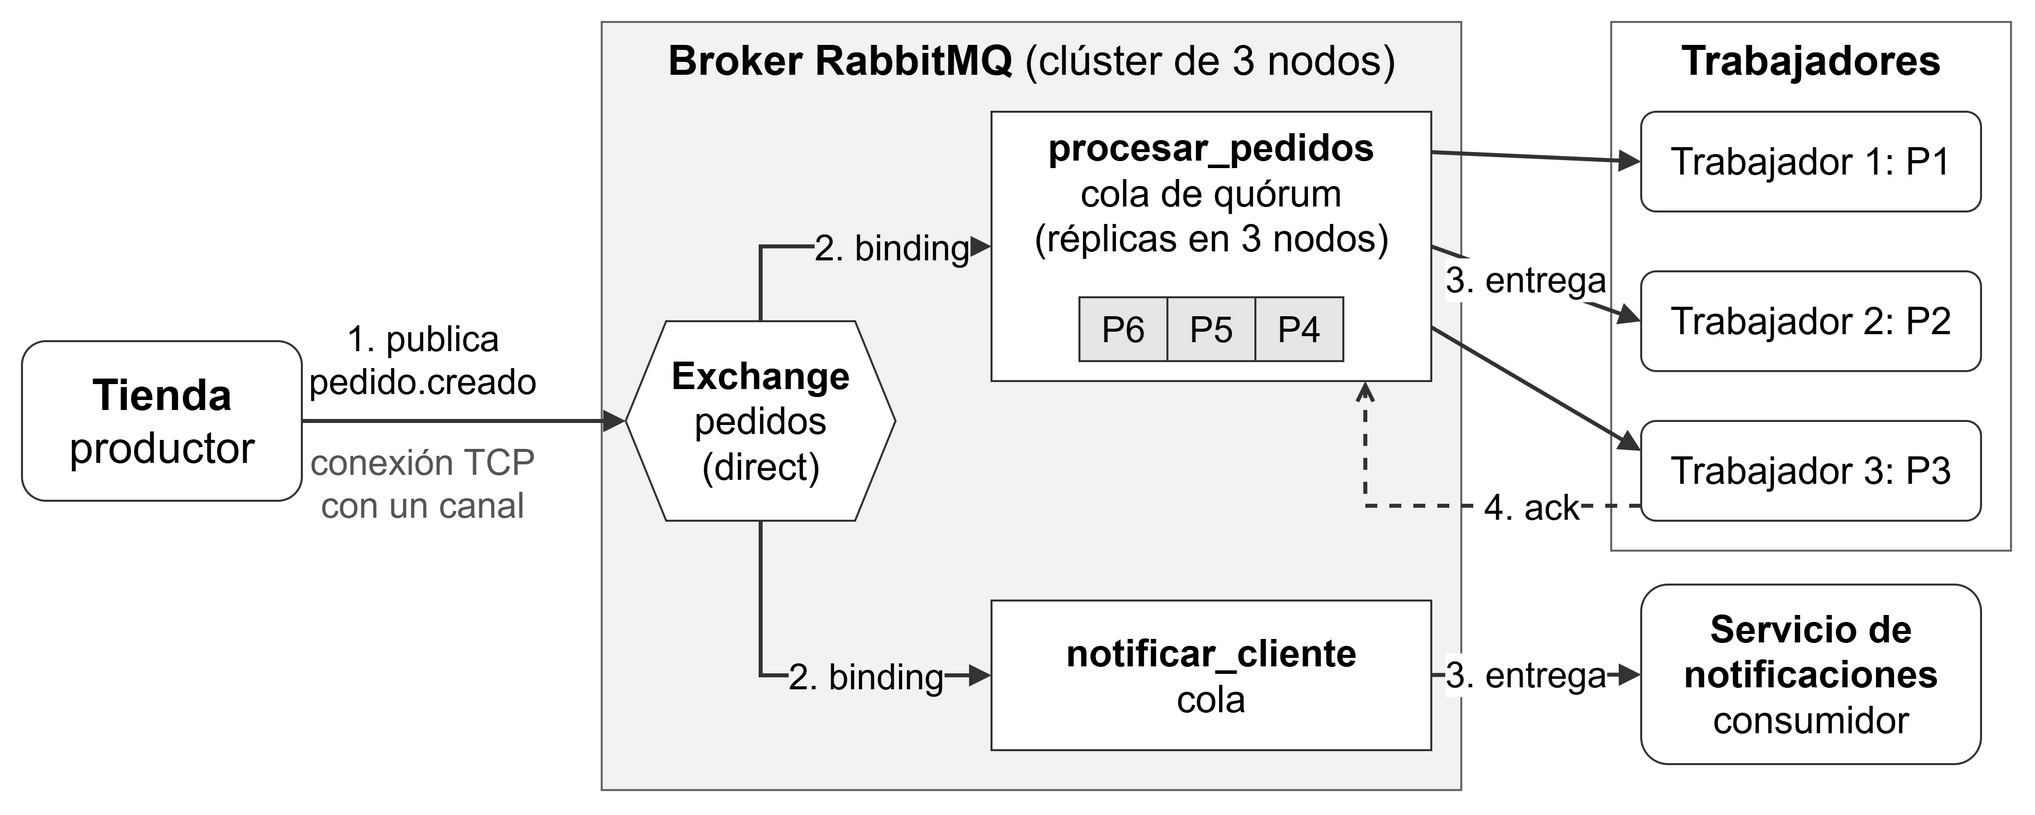
\includegraphics[width=\textwidth,height=0.68\textheight,keepaspectratio]{diagramas/arquitectura.png}

  \raggedright
  \footnotesize
  \begin{columns}[T]
    \begin{column}{0.48\textwidth}
      \begin{enumerate}
        \item La tienda publica con \texttt{pedido.creado}.
        \item El \textit{exchange} copia el pedido en ambas colas.
      \end{enumerate}
    \end{column}
    \begin{column}{0.48\textwidth}
      \begin{enumerate}
        \setcounter{enumi}{2}
        \item Cada pedido va a un solo trabajador.
        \item Sin \texttt{ack}, el pedido pasa a otro trabajador.
      \end{enumerate}
    \end{column}
  \end{columns}

  {\tiny Elaboración propia con base en
  \cite{rabbitmq2026amqp,rabbitmq2026queues,rabbitmq2026quorum}.}
\end{frame}
